%\graphicspath{{figures/Design/IPController/}}
\graphicspath{{figures/Rocket/design/}}

%\chapter{Design of the rocket Controller}\label{sec:IPController}
The goal of the controller is to balance the rocket body in an upright position. The system can be decomposed in a block diagram as shown in \autoref{fig:FinalChartName}.

\begin{figure}[htbp]
	\centering
	
	\includegraphics[width=\textwidth]{figures/Rocket/design/final_chart}
	\caption{Rocket transfer function.}
	\label{fig:FinalChartName}
	
\end{figure}

As seen in the modeling of the rocket and on \autoref{eq:RocketInitTf}, the system presents two poles in the origin of the pole-zero plot. 

\begin{subequations}
	\begin{flalign}
		& H = \frac{F_t \cdot L_{Cg} \cdot \frac{1}{M_r \cdot L_{Es}^2}}{s^2}	\label{eq:RocketInitTf} \\
		& H = \frac{3 \cdot 0.10 \cdot \frac{1}{0.180 \cdot 0.03^2}}{s^2}
	\end{flalign}
\end{subequations}
\startexplain
\explain{$F_t$ is the thruster force}{\si{\newton}}
\explain{$L_{Cg}$ is the distance from the thruster end to the center of gravity}{m}
\explain{$M_{Es}$ is the mass of the electronics stage}{\si{\kilo\gram}}
\explain{$L_{Es}$ is the distance from the electronics stage to the center of gravity}{\si{\meter}}
\stopexplain

Looking at the root locus of the system on \autoref{fig:Rinitialtf} shows the poles goes to infinity on the imaginary axis. This means that any oscillations or noise will never be damped solely by adding a gain. 
\begin{figure}[htbp]
\centering
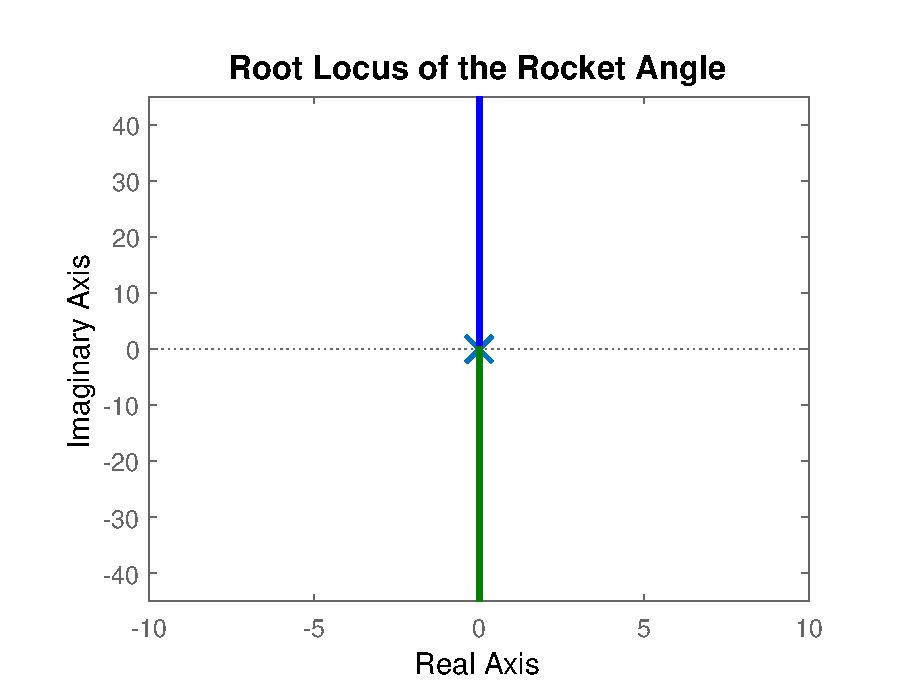
\includegraphics[width=0.7\textwidth]{figures/Rocket/design/initial_transfer_function_vf}
\caption{Root locus of the rocket angle transfer function.}
\label{fig:Rinitialtf}
\end{figure}

However the real system is also influenced by the servomotor. The transfer function of the servomotors is shown on \autoref{eq:TfServo}. 

\begin{subequations}
	\begin{flalign}
& H_s = \frac{1}{\uptau s+ 1}	\\
& H_s = \frac{1}{0.04s + 1}
\label{eq:TfServo}
	\end{flalign}
\end{subequations}
\startexplain
\explain{$\uptau$ is the time constant of the servomotors}{\si{\second}}
\stopexplain

This function then adds a pole to the initial transfer function, resulting in an unstable system. This is shown on \autoref{fig:SystemServo}.
\begin{figure}[htbp]
\centering
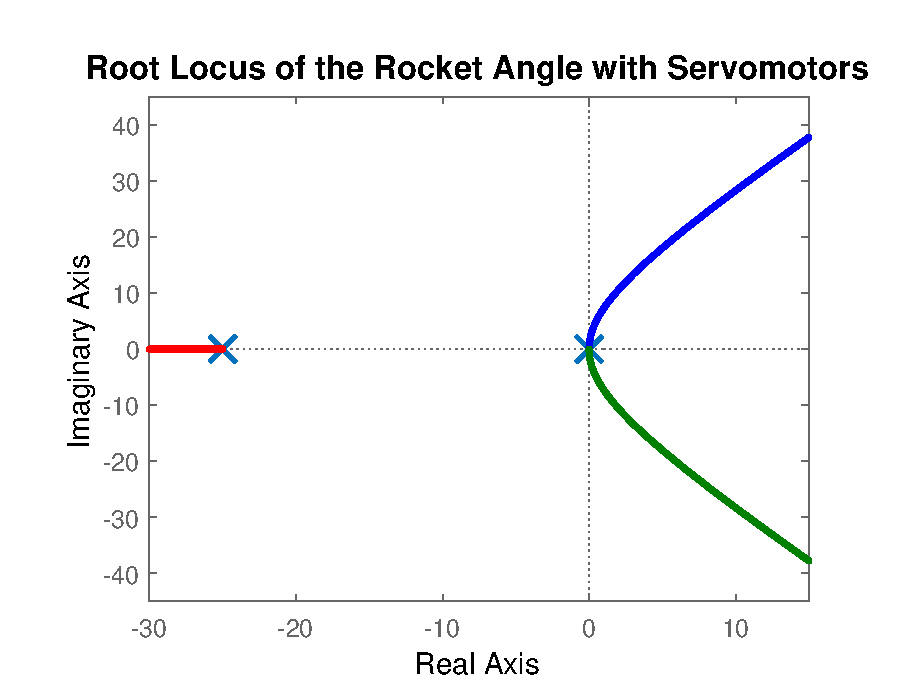
\includegraphics[width=0.7\textwidth]{figures/Rocket/design/tf_with_servo_vf}
\caption{Root locus of the system with the pole from the servomotors.}
\label{fig:SystemServo}
\end{figure}

This system could be controlled similarly to the inverted pendulum by doing cascade control. By having an inner loop that controls the servomotors as fast as possible the pole added can be assumed to have no effect. This would make the rocket control design nearly identical to the inverted pendulum by having an inner loop with a simple gain and an outer loop where a compensator in form of a zero needs to be added. 

The rocket built however doesn't have any sensors to measure the servomotors so this isn't an option. If the rocket was built differently this would be the preferred way to control it.

Instead an attempt to control the system using an inner loop.

\subsection{Controlling the Rocket Angle without Cascade Control}
To move the poles to the left half plane, a controller C1, adding a zero and a pole on the left side, is implemented to the rocket transfer function. If the zero is placed to close to the servo pole the loci will not be attracted to the real axis. Common practice recommends placing the pole at a location 20-40 times larger than the zero. Thus the zero of the controller is chosen experimentaly near the system in order to attract the poles, and the pole of the controller at a 40 times larger position. The controller C1 is shown on \autoref{eq:TfC1}.
\begin{equation}
C1 = \frac{s + 1.7}{s + 68}	\label{eq:TfC1}
\end{equation}

\begin{figure}[htbp]
\centering
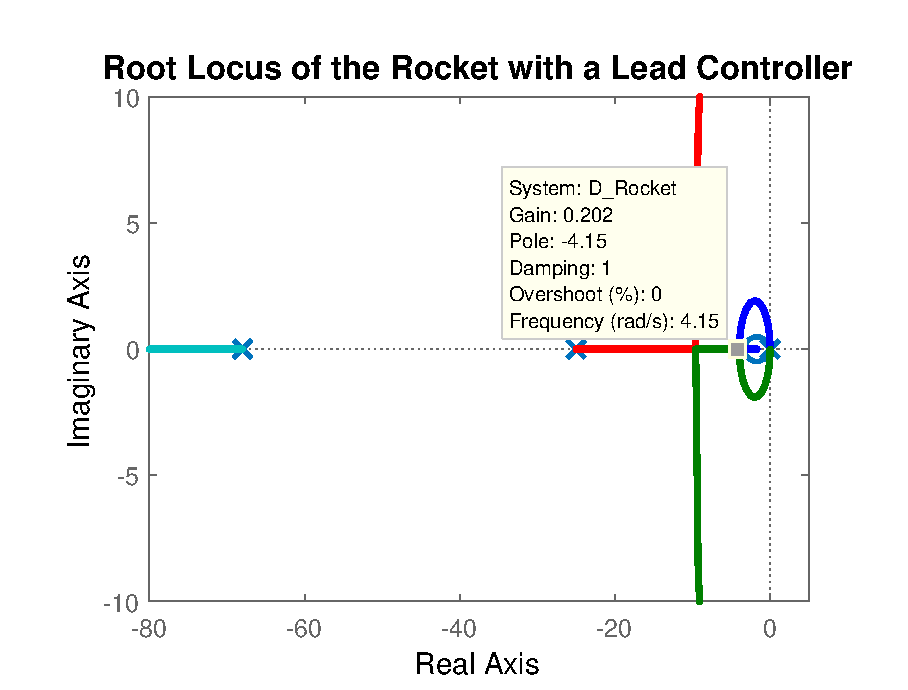
\includegraphics[width=\textwidth]{figures/Rocket/design/tf_with_controller_final_general}
\caption{Root locus of the system with a lead controller, C1, added.}
\label{fig:SystemC1}
\end{figure}

The rocket requires a fast settling time and rise time in order to act as soon as possible and control the rocket's stability. Lead compensaters enable the modulation of the rise time, but impact the overshoot. The overshoot is considered as an inferrior error, being in part countered by the play of the gimbal system. 
According to the specification the setling time should be faster than 1.5 second and the overshoot less than 25 per cent.

To improve the rise time, the gain is set at $0.404$ \si{\dB}. This value is chosen by observing the root locus and the gain of a set point, as shown on \autoref{fig:SystemC1C2Zoom}.  

				% Figure of chosen point
\begin{figure}[htbp]
	\centering
	
	\includegraphics[width=\textwidth]{figures/Rocket/design/tf_with_controller_final}
	\caption{Set point at the start of the circle.}
	\label{fig:SystemC1C2Zoom}
	
\end{figure}

To further improve the rise time and setling time of the rocket transfer function until the pysical and specification limits, the gain is doubled. 
The step response of the controlled rocket transfer function is shown on \autoref{fig:StepFinalRocket}.

\begin{figure}[htbp]
	\centering
	\includegraphics[width=\textwidth]{figures/Rocket/design/step_response_final}
	\caption{Step response of the rocket transfer function.}
	\label{fig:StepFinalRocket}
\end{figure}

The bodeplot of the controlled rocket transfer function is shown on \autoref{fig:BodePlotFinalTf}. The frequency correponds to a complete rotation of the servomotors. At low frequencies a delay is observed. However the system functions at low speed. This implies that the delay has a tempered effect on the system. Higher frequencies are not physicaly possible and do not need to be compensated.

				% Figure of final tf bodepoint
\begin{figure}[htbp]
	\centering
		\includegraphics[width=\textwidth]{figures/Rocket/design/bodeplot}
		\caption{Bodeplot of the rocket transfer function.}
		\label{fig:BodeplotFinalTf}
\end{figure}

The controlled rocket transfer function obtained is shown on equation \autoref{eq:RocketTfEqu} and  \autoref{fig:FinalChartNumbers}.

\begin{equation}    
H = 0.404 \cdot \frac{s + 1.7}{s + 68} \cdot \frac{1}{s \cdot \uptau + 1} \cdot \frac{F_t \cdot L_{Cg} \cdot \frac{1}{M_r \cdot L_{Es}^2}}{s^2}  
\end{equation}
\label{eq:RocketTfEqu}

\begin{figure}[htbp]
	\centering
	
	\includegraphics[width=\textwidth]{figures/Rocket/design/final_chart_number}
	\caption{Rocket transfer function.}
	\label{fig:FinalChartNumbers}
	
\end{figure}